\section{The read command}

\subsection{How it works}
\textcolor{blue}{\textbf{read}}: returns the bytes of the file. It takes in argument the path to the file.
First it checks if the path refers to a file and not a directory.\\

Then, we call the function \textit{file\_from\_path}. If it returns a value  equal to -1, that means the file doesn't exist. Else, we'll use the function \textit{file\_id} to get the index of the file in the \textit{file\_array}.\\

Thanks to the File struct, we can access easily to the content of the file with the member \textit{File.bytes}. Finally we print it in the standard output.\\
\begin{center}
    \begin{tabular}{cc}
        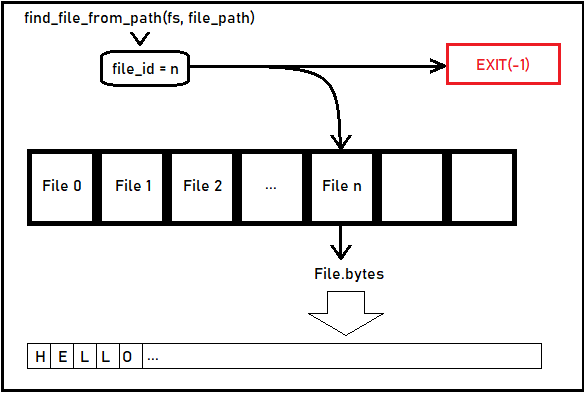
\includegraphics{figures/read.png}
    \end{tabular}
    \captionof{figure}{Reading a file (made with MS Paint)}
\end{center}

\newpage
\subsection{Testing}
\lstset{language=bash,caption={Read command},label=code:read-command}
\begin{lstlisting}
$ echo "Random string 123" > /tmp/foo.txt
$ vmhFS /tmp/tmpFS write /tmp/foo.txt /dir1/dir2/foo.txt
$ vmhFS /tmp/tmpFS read /dir1/dir2/foo.txt
$ vmhFS /tmp/tmpFS read /dir1/dir2/foo2.txt
\end{lstlisting}

\lstset{language=bash,caption={Command output},label=code:command-output}
\begin{lstlisting}
Write file /tmp/foo.txt to filesystem at: /dir1/dir2/foo.txt
Random string 123
File doesn't exist
\end{lstlisting}

\newpage